
In this section we will use \mRa-estimators for some specific families of probability distributions. As was stated above, results for normal model were already presented in  \cite{Vajda2009}, \cite{Demut2010}. Therefore we focused on exponential, Laplace, Cauchy and Weibull families. In case of these families we focused on deriving specific simple forms of estimator according to \eqref{eq:renEstimator} and also the form of influence function \eqref{eq:IF}.

\subsection{Laplace distribution} 
Here we use \mRa-estimators to estimate parameter $\theta = (\mu,\lambda)$ in Laplace model. Laplace probability density function can be written as 
\begin{equation}
	p_\theta = \frac{1}{2\lambda} e^{-\frac{|x-\mu|}{\lambda}}, \qquad \mu\in \mathbb{R},\, \lambda>0.
\end{equation}
For $\alpha = 0$ is the estimator \eqref{eq:renEstimator} equal to maximum likelihood estimator
\begin{align}
	\hat{\theta}_{\mathfrak{R}_0,n} & = \arg \max_{\theta \in \Theta} \frac{1}{n} \sum^n_{i=1} \ln \left[ \frac{1}{2\lambda}\exp \left[-\frac{|x_i-\mu|}{\lambda} \right] \right] \nonumber \\
	& =  \arg \max_{\theta \in \Theta} \left[ \ln \frac{1}{2\lambda} - \frac{1}{n} \sum^n_{i=1} \frac{|x_i-\mu|}{\lambda} \right].
\end{align}
Condition \eqref{eq:betaCond} holds for all $\beta>0$, therefore we can \mRa-estimator \eqref{eq:renEstimator} of parameters of Laplace distribution write for $\alpha>0$ as
\begin{equation}
	\hat{\theta}_{\mathfrak{R}_\alpha,n} = \arg \max_{\theta \in \Theta} \left[ (2\lambda)^{-\frac{\alpha}{1+\alpha}} \frac{1}{n} \sum_{i=1}^n \exp \left[-\alpha\frac{|x_i-\mu|}{\lambda} \right] \right].
	\label{renyi-formula-laplace}
\end{equation}
Via this formula we can estimate simultaneously both parameters $\mu, \lambda$ of the model. If one of the parameters is known and therefore there isn't need for it's estimation, we can simply fix it's value and maximize over the second parameter.

Here we present influence function for \mRa-estimator for Laplace model calculated from \eqref{eq:IF}. For the location estimator $(\hat{\theta} = \mu)$ with$\lambda$ known, we get influence function in the form

\begin{equation}
	\mathrm{IF}(x;T_{\mathfrak{R}_\alpha},\mu) = (1+\alpha )^{\frac{3}{2}} (x-\mu )  e^{-\frac{\alpha}{2} (x-\mu )^2}. % IF(x,mu)
	\label{IF-laplace-mu}
\end{equation}
If we switch the role of the parameters, meaning that we estimate the scale $\hat{\theta} = \lambda$, while fixing the $ \mu$, we get 
\begin{equation}
	\mathrm{IF}(x;T_{\mathfrak{R}_\alpha},\lambda) = (1 + \alpha)^2 \left(-\lambda + (1 + \alpha)|x-\mu|\right)  e^{-\frac{\alpha|x-\mu|}{\lambda}}	. % IF(x,sigma)
	\label{IF-laplace-lambda}
\end{equation}

\begin{figure}[htb]
\begin{center}
\begin{tabular}{c c c}
	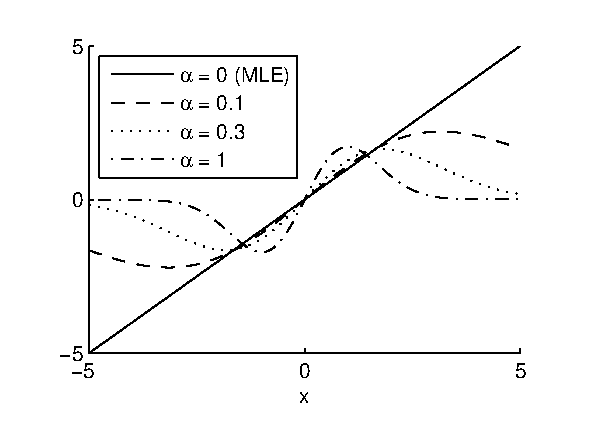
\epsfig{file=Laplace-IF-mu.eps, height=2.in} 
	&&
	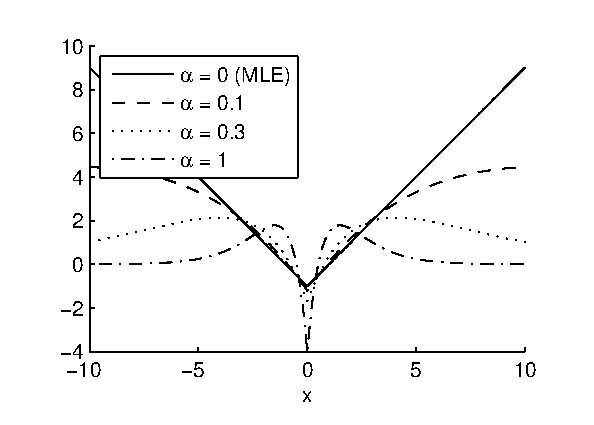
\epsfig{file=Laplace-IF-lambda.eps, height=2.in} 
	\\
	$\mathrm{IF}(x;T_{\mathfrak{R}_\alpha},\mu = 0) $ in case of known $\lambda = 1$ 
	&&
	$\mathrm{IF}(x;T_{\mathfrak{R}_\alpha},\lambda = 1)$ in case of known $\mu = 0$ 
	\\
\end{tabular}
\caption{Influence function of \mRa-estimators of parameters of Laplace distribution}
\label{fig:laplace-if}
\end{center}
%\label{fig:laplace-if}
\end{figure}

From \eqref{IF-laplace-mu} and \eqref{IF-laplace-lambda} we can see, that both influence functions are for $\alpha>0$ bounded, therefore B-robust. 

Moreover for both functions it holds that 

\begin{equation}
	\lim_{x \rightarrow \pm\infty} \mathrm{IF}(x;T_{\mathfrak{R}_\alpha},\cdot) = 0.
\end{equation}
 
\noindent Although the rejection points $\rho^*$ isn't finite, but the limits hold. We can see, that this convergence has exponential development in $\alpha$ due to the component  $e^{-\alpha x}$ in both functions. This means, that the estimator is more robust with higher value of $\alpha$. This can be also seen in the figure \ref{fig:laplace-if}, where the influence functions for both estimated parameters are shown separately for various $\alpha$.  We can see that maximum likelihood estimator $(\alpha = 0)$ isn't bounded and that the functions approach 0 faster with increasing $|x|$ for higher values of $\alpha$.

\subsection{Exponential distribution} 
Here we use \mRa-estimators to estimate parameter $\theta = (\mu,\lambda)$ in exponential distribution with probability density function 
\begin{equation}
	p_\theta = \frac{1}{\lambda} e^{-\frac{x-\mu}{\lambda}}, \qquad \mu\in \mathbb{R},\, \lambda>0, \, x\geq\mu.
\end{equation}
\noindent Exponential density's form is very similar to that of Laplace density. Below we will see, that even formulas for \mRa-estimators are very similar in both models. For $\alpha = 0$ we get \mRa-estimator in the form
\begin{align}
	\hat{\theta}_{\mathfrak{R}_0,n} & =  \arg \max_{\theta \in \Theta} \frac{1}{n} \sum^n_{i=1} \ln \left[ \frac{1}{\lambda}\exp \left[-\frac{x_i-\mu}{\lambda} \right] \right] \nonumber \\
	& =  \arg \max_{\theta \in \Theta} \left[ \ln \frac{1}{\lambda} - \frac{1}{n} \sum^n_{i=1} \frac{x_i-\mu}{\lambda} \right].
\end{align}

\noindent Condition \ref{eq:betaCond} holds again for all  $\beta>0$, therefore we can write \mRa-estimator for exponential family for $\alpha>0$ as
\begin{equation}
	\hat{\theta}_{\mathfrak{R}_\alpha,n} = \arg \max_{\theta \in \Theta} \lambda^{-\frac{\alpha}{1+\alpha}} \frac{1}{n}\sum_{i=1}^n \exp \left[-\alpha\frac{x_i-\mu}{\lambda} \right].
	\label{renyi-formula-exponential}
\end{equation}

We can see, that the difference to \eqref{renyi-formula-laplace} is only in the use of absolute value in Laplace model.

For  the estimator of location $\hat{\theta} = \mu$ in case of known $\lambda$, the influence function is the same as in the Laplace family $\eqref{IF-laplace-mu}$, therefore it holds

\begin{equation}
	\mathrm{IF}(x;T_{\mathfrak{R}_\alpha},\mu) = (1+\alpha )^{\frac{3}{2}} (x-\mu )  e^{-\frac{\alpha}{2} (x-\mu )^2}. % IF(x,mu)
	\label{IF-exponential-mu}
\end{equation}
If we estimate parameter of scale $\hat{\theta} = \lambda$ in case of known $ \mu $, we get formula
\begin{equation}
	\mathrm{IF}(x;T_{\mathfrak{R}_\alpha},\lambda) =	(1+\alpha )^2 \left( - \lambda +(1+ \alpha)(x-\mu)\right) e^{-\frac{\alpha (x-\mu)}{\lambda }}. % IF(x,lambda),
	\label{IF-exponential-lambda}
\end{equation}

\begin{figure}[htb]
\begin{center}
\begin{tabular}{c c c}
	\epsfig{file=Exp-IF-mu.eps, height=2.1in} 
	&&
	\epsfig{file=Exp-IF-lambda.eps, height=2.1in} 
	\\
	$\mathrm{IF}(x;T_{\mathfrak{R}_\alpha},\mu = 0) $ in case of known $\lambda = 1$
	&&
	$\mathrm{IF}(x;T_{\mathfrak{R}_\alpha},\lambda = 1)$ in case of known $\mu = 0$
	\\
\end{tabular}
\caption{Influence function of \mRa-estimators of parameters of exponential distribution}
\label{fig-exp-if}
\end{center}
\end{figure}

\noindent We can see from \eqref{IF-exponential-mu} and \eqref{IF-exponential-lambda} that for both functions it holds, that

\begin{equation}
	\lim_{x \rightarrow \pm\infty} \mathrm{IF}(x;T_{\mathfrak{R}_\alpha},\cdot) = 0,
\end{equation}
therefore outliers will be partially ignored due to the convergence of influence functions to 0. Again it holds, that the convergence is faster with greater $\alpha$, which can be seen in figure \ref{fig-exp-if}, as well as the fact, that the functions are bounded for all $\alpha >0$.

\subsection{Cauchy distribution} 


Dalším rozdělením, na které jsme použili Rényiho odhady, je Cauchyho s parametrem $\theta = (\mu,\sigma)$ a hustotou pravděpodobnosti
\begin{equation}
	p_\theta = \frac{1}{\pi\sigma} \left( 1 + \left( \frac{x-\mu}{\sigma} \right)^2 \right)^{-1}, \qquad \mu\in \mathbb{R},\, \sigma>0.
\end{equation}
Minimální $\mathfrak{R}_\alpha$-odhad je pro $\alpha=0$ roven
\begin{align}
	\hat{\theta}_{\mathfrak{R}_0,n} & = \arg \max_{\theta \in \Theta} \frac{1}{n} \sum^n_{i=1} \ln \left[  \frac{1}{\pi\sigma} \left( 1 + \left( \frac{x_i-\mu}{\sigma} \right)^2 \right)^{-1}   \right] \nonumber \\
	& =  \arg \max_{\theta \in \Theta} \left[ -\ln \pi\sigma - \frac{1}{n} \sum^n_{i=1} \ln \left[ 1 + \left( \frac{x_i-\mu}{\sigma} \right)^2 \right] \right],
\end{align}
který je shodný s maximálně věrohodným odhadem. Podmínka \eqref{eq:betaCond} platí tak jako v předchozích případech pro každé $\beta>0$. Pro $\alpha>0$ pak vychází minimální $\mathfrak{R}_\alpha$-odhad \eqref{eq:renEstimator} parametrů v Cauchyho modelu jako 

\begin{equation}
	\hat{\theta}_{\mathfrak{R}_\alpha,n} = \arg \max_{\theta \in \Theta} \left[ \sigma^{-\frac{\alpha}{1+\alpha}} \frac{1}{n} \sum_{i=1}^n \left( 1 + \left( \frac{x_i-\mu}{\sigma} \right)^2 \right)^{-\alpha} \right].
	\label{renyi-formula-cauchy}
\end{equation}

Influenční funkci \eqref{IF} pro minimální $\mathfrak{R}_\alpha$-odhady v Cauchyho rodině se nám podařilo dopočítat jen pro odhad parametru polohy $\theta = \mu$. Za předpokladu znalosti měřítka $\sigma$ má funkce tvar

\begin{equation}
	\mathrm{IF}(x;T_{\mathfrak{R}_\alpha},\mu) = \sqrt{\pi}\frac{\Gamma\left( 3 + \alpha \right)}{\Gamma\left( \frac{3}{2} + \alpha \right)} \left( \frac{\sigma^2}{\sigma^2 + (x-\mu)^2}\right)^{1+\alpha}(x-\mu).
	\label{IF-cauchy-mu}
\end{equation}

\noindent Z \eqref{IF-cauchy-mu} a obrázku \ref{fig:cauchy-if} je vidět, že influenční funkce je pro $\alpha>0$ omezená. Bod zamítání $\rho^*$ opět není konečný, ale pro $\alpha>0$ platí alespoň limita

\begin{equation}
	\lim_{x \rightarrow \pm\infty} \mathrm{IF}(x;T_{\mathfrak{R}_\alpha},\mu) = 0.
\end{equation}

\begin{figure}[htb]
\begin{center}
\begin{tabular}{c}
	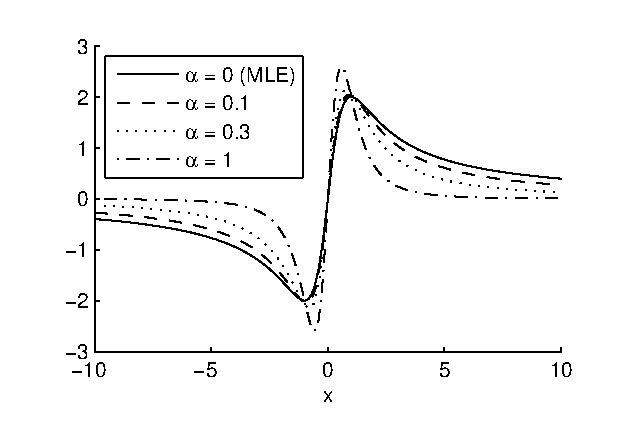
\epsfig{file=Cauchy-IF-mu.eps, height=2.6in} \\
	$\mathrm{IF}(x;T_{\mathfrak{R}_\alpha},\mu = 0) $ při $\sigma = 1$ známém
\end{tabular}
\caption{Influenční funkce {\mRao}ů pro Cauchyovo rozdělení}
\label{fig:cauchy-if}
\end{center}
\end{figure}

\noindent Podle vzorce \eqref{IF} se  nakonec podařilo dopočítat influenční funkci pro odhad měřítka $\theta = \sigma$ při znalosti polohy $\mu$. Následujícího výsledku bylo dosaženo výpočtem ve \texttt{Wolfram Mathematica}. Výsledný tvar je tedy

\begin{eqnarray}
\mathrm{IF}(x;T_{\mathfrak{R}_\alpha},\sigma) &=& -\left[4 \sqrt{\pi } (1+\alpha )^2 \sigma ^{2+\alpha } \left(\frac{\sigma }{(x-\mu )^2+\sigma ^2}\right)^{\alpha} \right. \nonumber\\
&&\left(\frac{1}{\sigma }+\frac{\alpha  \left(\frac{1}{\sigma }\right)^{\alpha } \sigma ^{-1+\alpha }}{1+\alpha }-\frac{2 \sigma }{(x-\mu )^2+\sigma ^2}\right) \left. \cos[\pi  \alpha ] \Gamma[\alpha ] \Gamma[1+\alpha ]  \frac{}{} \right] / \nonumber \\ %prázdný zlomek je tam kvůli roztažení koncové závorky
&&\left(4^{1-\alpha } \sqrt{\pi } \left(\frac{1}{\sigma }\right)^{\alpha } \sigma ^{\alpha } \left(-1+\alpha  \left(-1+\alpha  \left(-2+\left(\frac{1}{\sigma }\right)^{\alpha } \sigma ^{\alpha }\right)\right)\right) \right.\nonumber \\ 
&&\left. \cos[\pi  \alpha ] \Gamma[1+2 \alpha ]+1/(3 (3+4 \alpha  (2+\alpha )))\right. \nonumber \\
&& 8 \pi  (1+\alpha ) \left(-1+\alpha  (1+\alpha )^2\right) \Gamma[\alpha ] \nonumber \\
&& \left(6 (1+\alpha ) ^r_2\mathrm{F}_1\left[\frac{1}{2},2,\frac{1}{2}-\alpha ,1\right]-4^{-\alpha } \Gamma[4+2 \alpha ] \right. \nonumber \\
&& \left. \left. ^r_2\mathrm{F}_1\left[\frac{1}{2}+\alpha ,1+\alpha ,-\frac{1}{2}+\alpha ,1\right]\right)\right),
\end{eqnarray}

\noindent kde $^r_2\mathrm{F}_1[a,b;c;z]$ je regularizovaná hypergeometrická funkce 

\begin{equation}
	^r_2\mathrm{F}_1[a,b;c;z] = {\frac{1}{\Gamma[c]}} {_2\mathrm{F}_1}[a,b;c;z],
\end{equation}
přičemž hypergeometrická funkce je definovaná vztahem
\begin{equation}
	{_2\mathrm{F}_1}[a,b;c;z]=\sum _{n=0}^{\infty } \frac{(a)_n (b)_n z^n}{ (c)_n n!}, \qquad |z|<1, \, \text{ nebo } \, (|z|=1\l  \,\text{a} \,  c>a+b),
\end{equation}

\noindent kde $(a)_n$ je Pochhammerův symbol definovaný

\begin{equation}
(a)_n=\prod _{k=0}^{n-1} (a+k), \qquad n \in \mathbb{N}.
\end{equation}

\noindent Kvůli definici hypergeometrické funkce tato influenční funkce však nemá smysl, protože z definičních podmínek nám vychází $\frac{1}{2}+\alpha  + 1+\alpha < -\frac{1}{2}+\alpha $, tedy $\alpha < -2$, což ale odporuje výběru $\alpha>0$ z věty \ref{renyi-veta}. 

\subsection{Weibull distribution} 

Posledním zpracovávaným rozdělením, bylo tříparametriké Weibullovo s parametrem $\theta = (\mu,\lambda,k)$ a hustotou pravděpodobnosti
\begin{equation}
	p_\theta =  \frac{k}{\lambda} \left( \frac{x-\mu}{\lambda} \right)^{k-1} \exp \left[ -\left( \frac{x-\mu}{\lambda} \right)^k \right], \qquad \mu \in \mathbb{R}, \, \lambda>0, \, k>0, \, x \geq \mu.
\end{equation}

\noindent Pro $\alpha = 0$ je minimální Rényiho odhad roven

\begin{align}
	\hat{\theta}_{\mathfrak{R}_0,n} & = \arg \max_{\theta \in \Theta} \frac{1}{n} \sum^n_{i=1} \ln \left[ \frac{k}{\lambda} \left( \frac{x_i-\mu}{\lambda} \right)^{k-1} 
	\exp \left[ -\left( \frac{x_i-\mu}{\lambda} \right)^k \right]\right] \nonumber \\
	&=\arg \max_{\theta \in \Theta}\left[ \ln \frac{k}{\lambda} + \frac{k-1}{n} \sum^n_{i=1} \ln \left[  \frac{x_i-\mu}{\lambda} \right] - 
	\frac{1}{n} \sum^n_{i=1} \left(  \frac{x_i-\mu}{\lambda} \right)^k \right].
\end{align}

\noindent Podmínka \ref{eq:betaCond} opět platí pro každé $\beta>0$. Pro $\alpha>0$ pak vychází minimální $\mathfrak{R}_\alpha$-odhad \eqref{eq:renEstimator} parametrů ve Weibullově modelu ve tvaru

\begin{eqnarray}
	\hat{\theta}_{\mathfrak{R}_\alpha,n} & = & \arg \max_{\theta \in \Theta} \left( \frac{k}{\lambda} \right)^\frac{\alpha}{1+\alpha} (1+\alpha)^{\frac{\alpha}{1+\alpha}\frac{1+\alpha+k}{k}} 
	\Gamma\left(\frac{1+\alpha+k}{k}\right)^{-\frac{\alpha}{1+\alpha}} \nonumber \\
	&& \frac{1}{n}\sum_{i=1}^n \left( \frac{x_i-\mu}{\lambda}\right)^{\alpha(k-1)} \exp\left[-\alpha \left(\frac{x_i-\mu}{\lambda}\right)^k\right].
\end{eqnarray}

\noindent Kvůli použití $\Gamma$-funkce dostáváme dodatečnou podmínku $1+\alpha+k>0$, tedy $\alpha + k > -1$. Tato podmínka je ale splněna automaticky, protože jsou oba parametry kladné. 

Influenční funkce $\eqref{IF}$ pro odhad polohy $\theta = \mu$ pří známých parametrech $\lambda, k $  má tvar

\begin{equation}
	\mathrm{IF}(x;T_{\mathfrak{R}_\alpha},\mu) = \frac{(1+\alpha )^{\frac{-2-\alpha +k (3+\alpha )}{k}} \lambda \left(1+k \left(-1+\left(\frac{x-\mu }{\lambda }\right)^k\right)\right) 
	 \left(\frac{x-\mu }{\lambda }\right)^{\alpha k-\alpha-1}\exp \left[-\alpha\left(\frac{x-\mu }{\lambda }\right)^k\right]}
	 {(-1+k) (-1+k+k \alpha ) \Gamma\left[\frac{-2+k+(-1+k) \alpha }{k}\right]}.
	\label{IF-weibull-mu}
\end{equation}

\noindent Z použití $\Gamma$-funkce vyplývá podmínka $k > 1 + \frac{1}{1+\alpha}$, tedy $(\forall \alpha> 0) (k > 1)$. Pro $\alpha > 0$ opět kvůli exponenciálnímu členu platí

\begin{equation}
	\lim_{x \rightarrow \pm\infty} \mathrm{IF}(x;T_{\mathfrak{R}_\alpha},\mu) = 0.
\end{equation}

\begin{figure}[!htb]
\begin{center}
\begin{tabular}{cc}
	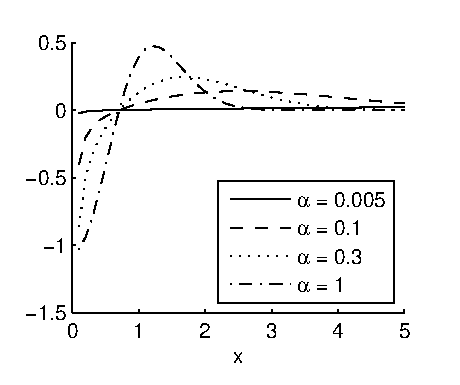
\epsfig{file=Weib-IF-mu.eps, height=2.2in} & 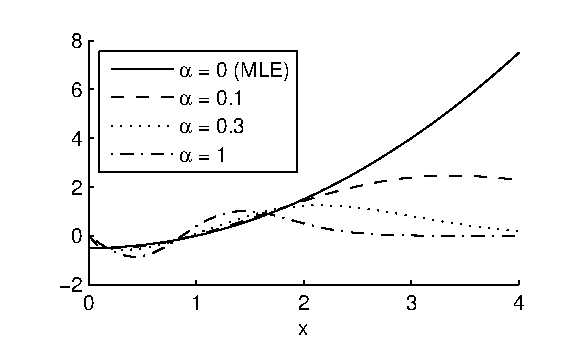
\epsfig{file=Weib-IF-lambda.eps, width=3.2in}
	\\	
	$\mathrm{IF}(x;T_{\mathfrak{R}_\alpha},\mu = 0) $, známé $\lambda = 1, \: k = 2$ & $\mathrm{IF}(x;T_{\mathfrak{R}_\alpha},\lambda = 1) $, známé $\mu = 0, \: k = 2$
\end{tabular}
\caption{Influenční funkce {\mRao}ů $\mu$ a $\lambda$ Weibullovo rozdělení}
\label{figJK:weibull-if}
\end{center}
\end{figure}

\noindent Na obrázku \ref{figJK:weibull-if} je vidět, že je influenční funkce opět omezená. V obrázku není vykreslena funkce pro $\alpha = 0$, protože pro $k=2$ je nutné použít $\alpha >0$.
Pro odhad měřítka $\theta = \lambda$ při známých $\mu, k$ má influenční funkce tvar

\begin{equation}
	\mathrm{IF}(x;T_{\mathfrak{R}_\alpha},\lambda) = \frac{(1+\alpha )^{2+\alpha -\frac{\alpha }{k}} \lambda  \left(\alpha +k (1+\alpha ) \left(-1+\left(\frac{x-\mu }{\lambda }\right)^k\right)\right)
	\left(\frac{x-\mu}{\lambda}\right)^{\alpha k-\alpha} \exp \left[-\alpha\left(\frac{x-\mu}{\lambda}\right)^k\right]}
	{k^2 \Gamma\left[2+\alpha -\frac{\alpha }{k}\right]}.
	\label{IF-weibull-lambda}
\end{equation}

\noindent Opět z použití $\Gamma$-funkce vyplývá $k>\frac{\alpha}{2+\alpha}$. Funkce pro $\alpha > 0$ a $x\rightarrow \pm \infty$ konverguje k $0$ a je omezená. což je vidět i na obrázku \ref{figJK:weibull-if}. Pro odhad parametru $\theta = k$ jsme influenční funkci opět počítali ve \texttt{Wolfram Mathematica}. Funkce vyšla ve tvaru

\begin{eqnarray}
	\mathrm{IF}(x;T_{\mathfrak{R}_\alpha},k)& = &\left(k^2 (1+\alpha )^{2+\alpha -\frac{\alpha }{k}} \left(e^{-\left(\frac{x-\mu }{\lambda }\right)^k} \left(\frac{x-\mu }{\lambda }\right)^{-1+k}\right)^{\alpha } \right. \nonumber \\
	&& \left(\alpha  \text{ln}[1+\alpha ]+k \left(1-k (1+\alpha ) \left(-1+\left(\frac{x-\mu }{\lambda }\right)^k\right)\right.\right. \nonumber \\
	&& \left.\left.\left.\left.\text{ln}\left[\frac{x-\mu }{\lambda }\right]\right)-\alpha  \psi\left[0,1+\alpha -\frac{\alpha }{k}\right]\right)\right)\right/ \nonumber \\
	&& \left(\Gamma\left[1+\alpha -\frac{\alpha }{k}\right] (k (k+\ln[1+\alpha ] \right.  \\
	&& (-2 k+2 \alpha +(k+(-1+k) \alpha ) \ln[1+\alpha ]))-2 k (-k+\alpha + \nonumber \\
	&& (k+(-1+k) \alpha )\ln[1+\alpha ]) \psi\left[0,1+\alpha -\frac{\alpha }{k}\right]+k (k+(-1+k) \alpha ) \nonumber \\
	&& \left.\left.\psi\left[0,1+\alpha -\frac{\alpha }{k}\right]^2+\left(k^2+(-1+k) k \alpha +\alpha ^2\right) \psi\left[1,1+\alpha -\frac{\alpha }{k}\right]\right)\right), \nonumber
	\label{IF-weibull-k}
\end{eqnarray}

\noindent kde $\psi(n,z)$ je $(n+1)-$tá derivace logaritmu $\Gamma(z)$, tedy

\begin{equation}
	\psi(n,z) = \frac{\mathrm{d}^{n+1}}{\mathrm{d}z^{n+1}} \ln \Gamma(z).
\end{equation}

\noindent Kvůli použití $\Gamma$-funkce vzniká podmínka $k > \frac{\alpha}{1+\alpha}$. Funkce je pro $\alpha>0$ opět omezená a pro $x$ rostoucí nade všechny meze konverguje k 0. Na obrázku \ref{figJK:weibull2-if} je patrné, že tento odhad bude fungovat kvůli velké absolutní hodnotě influenční funkce lépe pro větší hodnoty $\alpha$.

\begin{figure}[htb]
\begin{center}
\begin{tabular}{cc}	
	\multicolumn{2}{c}{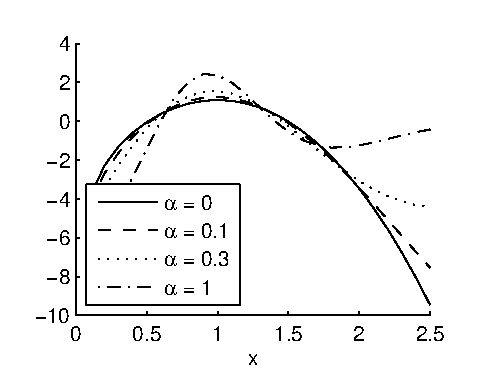
\epsfig{file=Weib-IF-k.eps, height=2.5in}}
	\\
	\multicolumn{2}{c}{$\mathrm{IF}(x;T_{\mathfrak{R}_\alpha},k = 2) $, známé $\mu = 0, \: \lambda = 1$}
\end{tabular}
\caption{Influenční funkce {\mRao}u $k$ pro Weibullovo rozdělení}
\label{figJK:weibull2-if}
\end{center}
\end{figure}



 


